\newpage
\subsection{Caso d'uso UC 2: Utilizzo di bolle predefinite dell'SDK.}
\label{Caso d'uso UC 2: Utilizzo di bolle predefinite dell'SDK.}
\begin{figure}[ht]
	\centering
	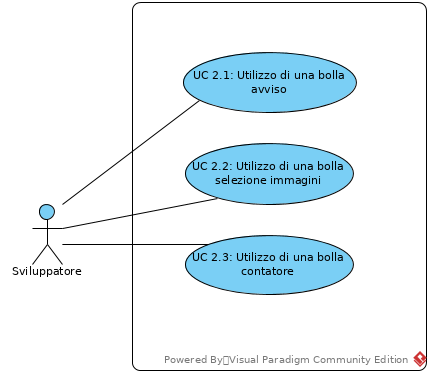
\includegraphics[scale=0.60]{Usecases/img/UC2.png}
	\caption{Caso d'uso UC 2: Utilizzo di bolle predefinite dell'SDK.}
\end{figure}

\FloatBarrier
\begin{itemize}
\item \textbf{Attori:} Sviluppatore.
\item \textbf{Descrizione:} Lo sviluppatore vuole utilizzare una bolla predefinita presente nell'SDK ovvero una tra le seguenti:
\begin{itemize}
\item Bolla avviso.
\item Bolla testo markdown.
\item Bolla lista.
\end{itemize} 
\item \textbf{Precondizione:} Lo sviluppatore vuole utilizzare una bolla predefinita presente nell'SDK. 
\item \textbf{Postcondizione:} Lo sviluppatore ha utilizzato una delle bolle predefinite presenti nella libreria di \progetto.
\item \textbf{Scenario principale:}
	\begin{itemize}
	\item{Utilizzo di una bolla avviso (UC 2.1).}
	\item{Utilizzo di una bolla testo markdown (UC 2.2).}
	\item{Utilizzo di una bolla lista (UC 2.3).}
	\end{itemize}
\end{itemize}